% ============================================== %
%%%%%%%%%%%%%%%%%%%% PREAMBLE %%%%%%%%%%%%%%%%%%%%
% ============================================== %
\documentclass[a4paper,11pt]{article}

\usepackage[main=vietnamese,english]{babel}
\usepackage[utf8]{inputenc}

\usepackage{pdfpages}
\usepackage{latexsym}
\usepackage{geometry}
\usepackage{titlesec}
\usepackage{enumitem}
\usepackage{hyperref}
\usepackage{fontawesome5}

% ----- Sections formatting
\geometry{margin=9mm, includefoot}
\pagestyle{empty}
\urlstyle{same}
\raggedbottom
\raggedright
\titleformat{\section}{\vspace{-4pt}\scshape\raggedright\large}{}{0em}{}[\color{black}\titlerule \vspace{-5pt}]
\pdfminorversion=6
%

% ----- Custom commands -----
\newcommand{\resumeItem}[2]{
  \item\small{
    \textbf{#1}{: #2 \vspace{-2pt}}
  }
}
\newcommand{\resumeSubheading}[4]{
  \vspace{-1pt}\item
    \begin{tabular*}{0.97\textwidth}{l@{\extracolsep{\fill}}r}
      \textbf{#1} & #2 \\
      \textit{\small#3} & \textit{\small #4} \\
    \end{tabular*}\vspace{-5pt}
}
\newcommand{\resumeSubItem}[2]{\resumeItem{#1}{#2}\vspace{-4pt}}
\renewcommand{\labelitemii}{$\circ$}
\newcommand{\resumeSubHeadingListStart}{\begin{itemize}[leftmargin=*]}
\newcommand{\resumeSubHeadingListEnd}{\end{itemize}}
\newcommand{\resumeItemListStart}{\begin{itemize}}
\newcommand{\resumeItemListEnd}{\end{itemize}\vspace{-5pt}}
\newcommand{\coverLetterHeader}{
    \small{
        Tường-Minh (Mike) Võ\\
        Thành phố Hồ Chí Minh, Việt Nam\\
        (+84)-385-892-705\\
        \href{miketvo@outlook.com}{miketvo@outlook.com}
    }
    \par\noindent\hrulefill
}
\newcommand{\p}[1]{#1\\\vspace{6pt}}
%
% ============================================== %


% ============================================== %
%%%%%%%%%%%%%%%%%%%%%% BODY %%%%%%%%%%%%%%%%%%%%%%
% ============================================== %
\begin{document}

% ----- HEADING -----
\begin{tabular*}{\textwidth}{l@{\extracolsep{\fill}}r}
  \textbf{Tường-Minh (Mike) Võ} & Email: \href{mailto:miketvo@outlook.com}{miketvo@outlook.com}\\
  \href{https://github.com/miketvo}{\faGithub\space miketvo} $|$ \href{https://www.linkedin.com/in/miketvo/}{\faLinkedin\space miketvo} $|$ \href{https://miketvo.com/}{\faGlobe\space miketvo.com} & Mobile: (84)-385-892-705\\
\end{tabular*}
\hrule height 2pt
%

% ----- EDUCATION -----
\section{Học Vấn}
  \resumeSubHeadingListStart
    \resumeSubheading
      {Đại học RMIT Việt Nam}{Thành phố Hồ Chí Minh, Việt Nam}
      {Cử nhân Công nghệ Thông tin về Trí tuệ Nhân tạo; GPA: 3.50}{10/2020 -- Tốt nghiệp: 03/2025}
    \resumeSubheading
      {Seattle Central College}{Seattle, WA, Hoa Kỳ}
      {Associate of Liberal Arts and Sciences; GPA: 3.00}{9/2016 -- 10/2017}
  \resumeSubHeadingListEnd

% ----- RELEVANT COURSEWORK -----
\section{Môn Học Liên Quan}
  Phát triển Ứng dụng Full-stack,
  Phát triển Ứng dụng Web,
  Ứng dụng Cơ sở dữ liệu,
  Cấu trúc Dữ liệu và Giải thuật,
  Xây dựng Hệ thống CNTT,
  Thiết kế Phần mềm,
  Quản lý Dự án Kỹ thuật Phần mềm
%

% ----- PROJECTS -----
\section{Dự Án}
  \resumeSubHeadingListStart

    \resumeSubheading
      {Bàn phím ảo mã nguồn mở Tiếng Việt cho phầm mềm bộ gõ Keyman}{}
      {\href{https://github.com/miketvo/keyboards}{\faGithub\space miketvo/keyboards} $|$ \href{https://keyman.com/keyboards/vietnamese_telex}{\faGlobe\space Keyman - Vietnamese Telex} $|$ \href{https://keyman.com/keyboards/vietnamese_vni}{\faGlobe\space Keyman - Vietnamese VNI}}{}
      \resumeItemListStart
        \resumeItem{Ngôn ngữ và Framework}
          {Python, Keyman Keyboard Language}
        \resumeItem{Bộ tạo phím tắt tiếng Việt toàn diện}
          {Sử dụng ngôn ngữ Python để tạo ra bộ cấu hình phím tắt Telex và VNI dựa trên phân tích âm tiết theo từ điển tiếng Việt thu thập qua internet.}
        \resumeItem{Hợp tác mã nguồn mở}
          {Hợp tác thông qua GitHub với các developer, admin, và cộng đồng người dùng Keyman để giải quyết bug và deploy hai bàn phím ảo trên kiến trúc của bộ gõ Keyman.}
        \resumeItem{Triển khai}
          {Cả phiên bản Telex và VNI tổng đạt được hơn 35,000 lượt tải về trên trang web Keyman.}
      \resumeItemListEnd

    \resumeSubheading
      {Imdupes}{}
      {Open-source versatile image deduplicator inspired by fdupes $|$ \href{https://github.com/miketvo/imdupes}{\faGithub\space miketvo/imdupes}}{}
      \resumeItemListStart
        \resumeItem{Ngôn ngữ và Framework}
          {Python, PyInstaller, Pillow, NumPy, Python unittest}
        \resumeItem{Phát triển thuật toán Perceptual Hashing mới}
          {Đạt được khả năng phân biệt hiệu suất cao cho nhiều loại và format hình ảnh bằng cách phát triển một thuật toán Perceptual Hashing cho hình ảnh thông qua kết hợp Perceptual Hashing truyền thống và phân tích Histogram màu.}
        \resumeItem{Triển khai}
          {Triển khai thành công ứng dụng trên các trình quản lý gói Homebrew và Scoop để cài đặt đa nền tảng nhanh chóng và dễ dàng trên MacOS, Linux và Windows.}
      \resumeItemListEnd

    \resumeSubheading
      {DsvCol}{}
      {Open-source cross-platform CLI-application pretty-printing delimiter separated value files $|$ \href{https://github.com/miketvo/dsvcol}{\faGithub\space miketvo/dsvcol}}{}
      \resumeItemListStart
        \resumeItem{Ngôn ngữ và Framework}
          {C, CMake, Bash, PowerShell}
      \resumeItemListEnd

    \resumeSubheading
      {Online Client Portfolio}{}
      {\href{https://duonghanhi.netlify.app/}{\faGlobe\space duonghanhi.netlify.app}}{}
      \resumeItemListStart
        \resumeItem{Ngôn ngữ và Framework}
          {JavaScript, Gatsby, PostCSS}
        \resumeItem{Thiết kế UI/UX}
          {Áp dụng phương thức Agile, làm việc online với khách hàng để thiết kế và phát triển một website với UI và trải nghiệm người dùng tối ưu, thân thiện, khớp với thương hiệu và chuẩn SEO}
      \resumeItemListEnd

    \resumeSubheading
      {Web Game}{}
      {\href{https://miketvo.github.io/404-page.html}{\faGlobe\space miketvo.github.io/404-page}}{}
      \resumeItemListStart
        \resumeItem{Ngôn ngữ và Framework}
          {JavaScript, Phaser 3, Box2D, Webpack}
        \resumeItem{Lãnh đạo và làm việc nhóm}
          {Giúp đỡ dưới vai trò trưởng nhóm các thành viên nhóm phát triển ứng dụng game HTML trên trình duyệt web thay thế cho trang 404 NOT FOUND. Host thông qua GitHub Pages.}
      \resumeItemListEnd

    \resumeSubheading
      {Mô hình Dự đoán Sốc nhiễm khuẩn}{}
      {\href{https://github.com/miketvo/rmit2023a-cosc2753-assignment1}{\faGithub\space miketvo/rmit2023a-cosc2753-assignment1} $|$ \href{https://www.kaggle.com/datasets/chaunguynnghunh/sepsis/}{\faDatabase\space Dataset: Kaggle - chaunguynnghunh/sepsis}}{}
      \resumeItemListStart
        \resumeItem{Ngôn ngữ và Framework}
          {Python, Scikit-Learn, Pandas, Seaborn}
        \resumeItem{Điểm F1}
          {Đạt được điểm $F_1$ là 0.86 thông qua xây dựng và áp dụng thuật toán Bagged Tree và pipeline xử lý và sàng lọc dữ liệu.}
      \resumeItemListEnd

  \resumeSubHeadingListEnd
%

% ----- SKILLS -----
\section{Kỹ Năng}
  \resumeSubHeadingListStart
    \resumeSubItem{Lập trình}
      {Python, SQL, Java, C/C++, JavaScript, PHP, HTML/CSS, Lua, Bash, Batch, Powershell, TeX}
    \resumeSubItem{Công nghệ}
      {ReactJS, GatsbyJS, NextJS, Vite, ExpressJS, MySQL, MongoDB, JUnit, Tensorflow, Keras, Pandas}
    \resumeSubItem{Công cụ}
      {Jira, Git, Vim, Visual Studio Code, Linux, Jupyter Lab, Jupyter Notebook, Jetbrains IDEs}
    \resumeSubItem{Ngôn ngữ}
      {Tiếng Việt (Bản ngữ), Tiếng Anh (Trình độ song ngữ)}
  \resumeSubHeadingListEnd
%

% ----- TRANSCRIPT -----
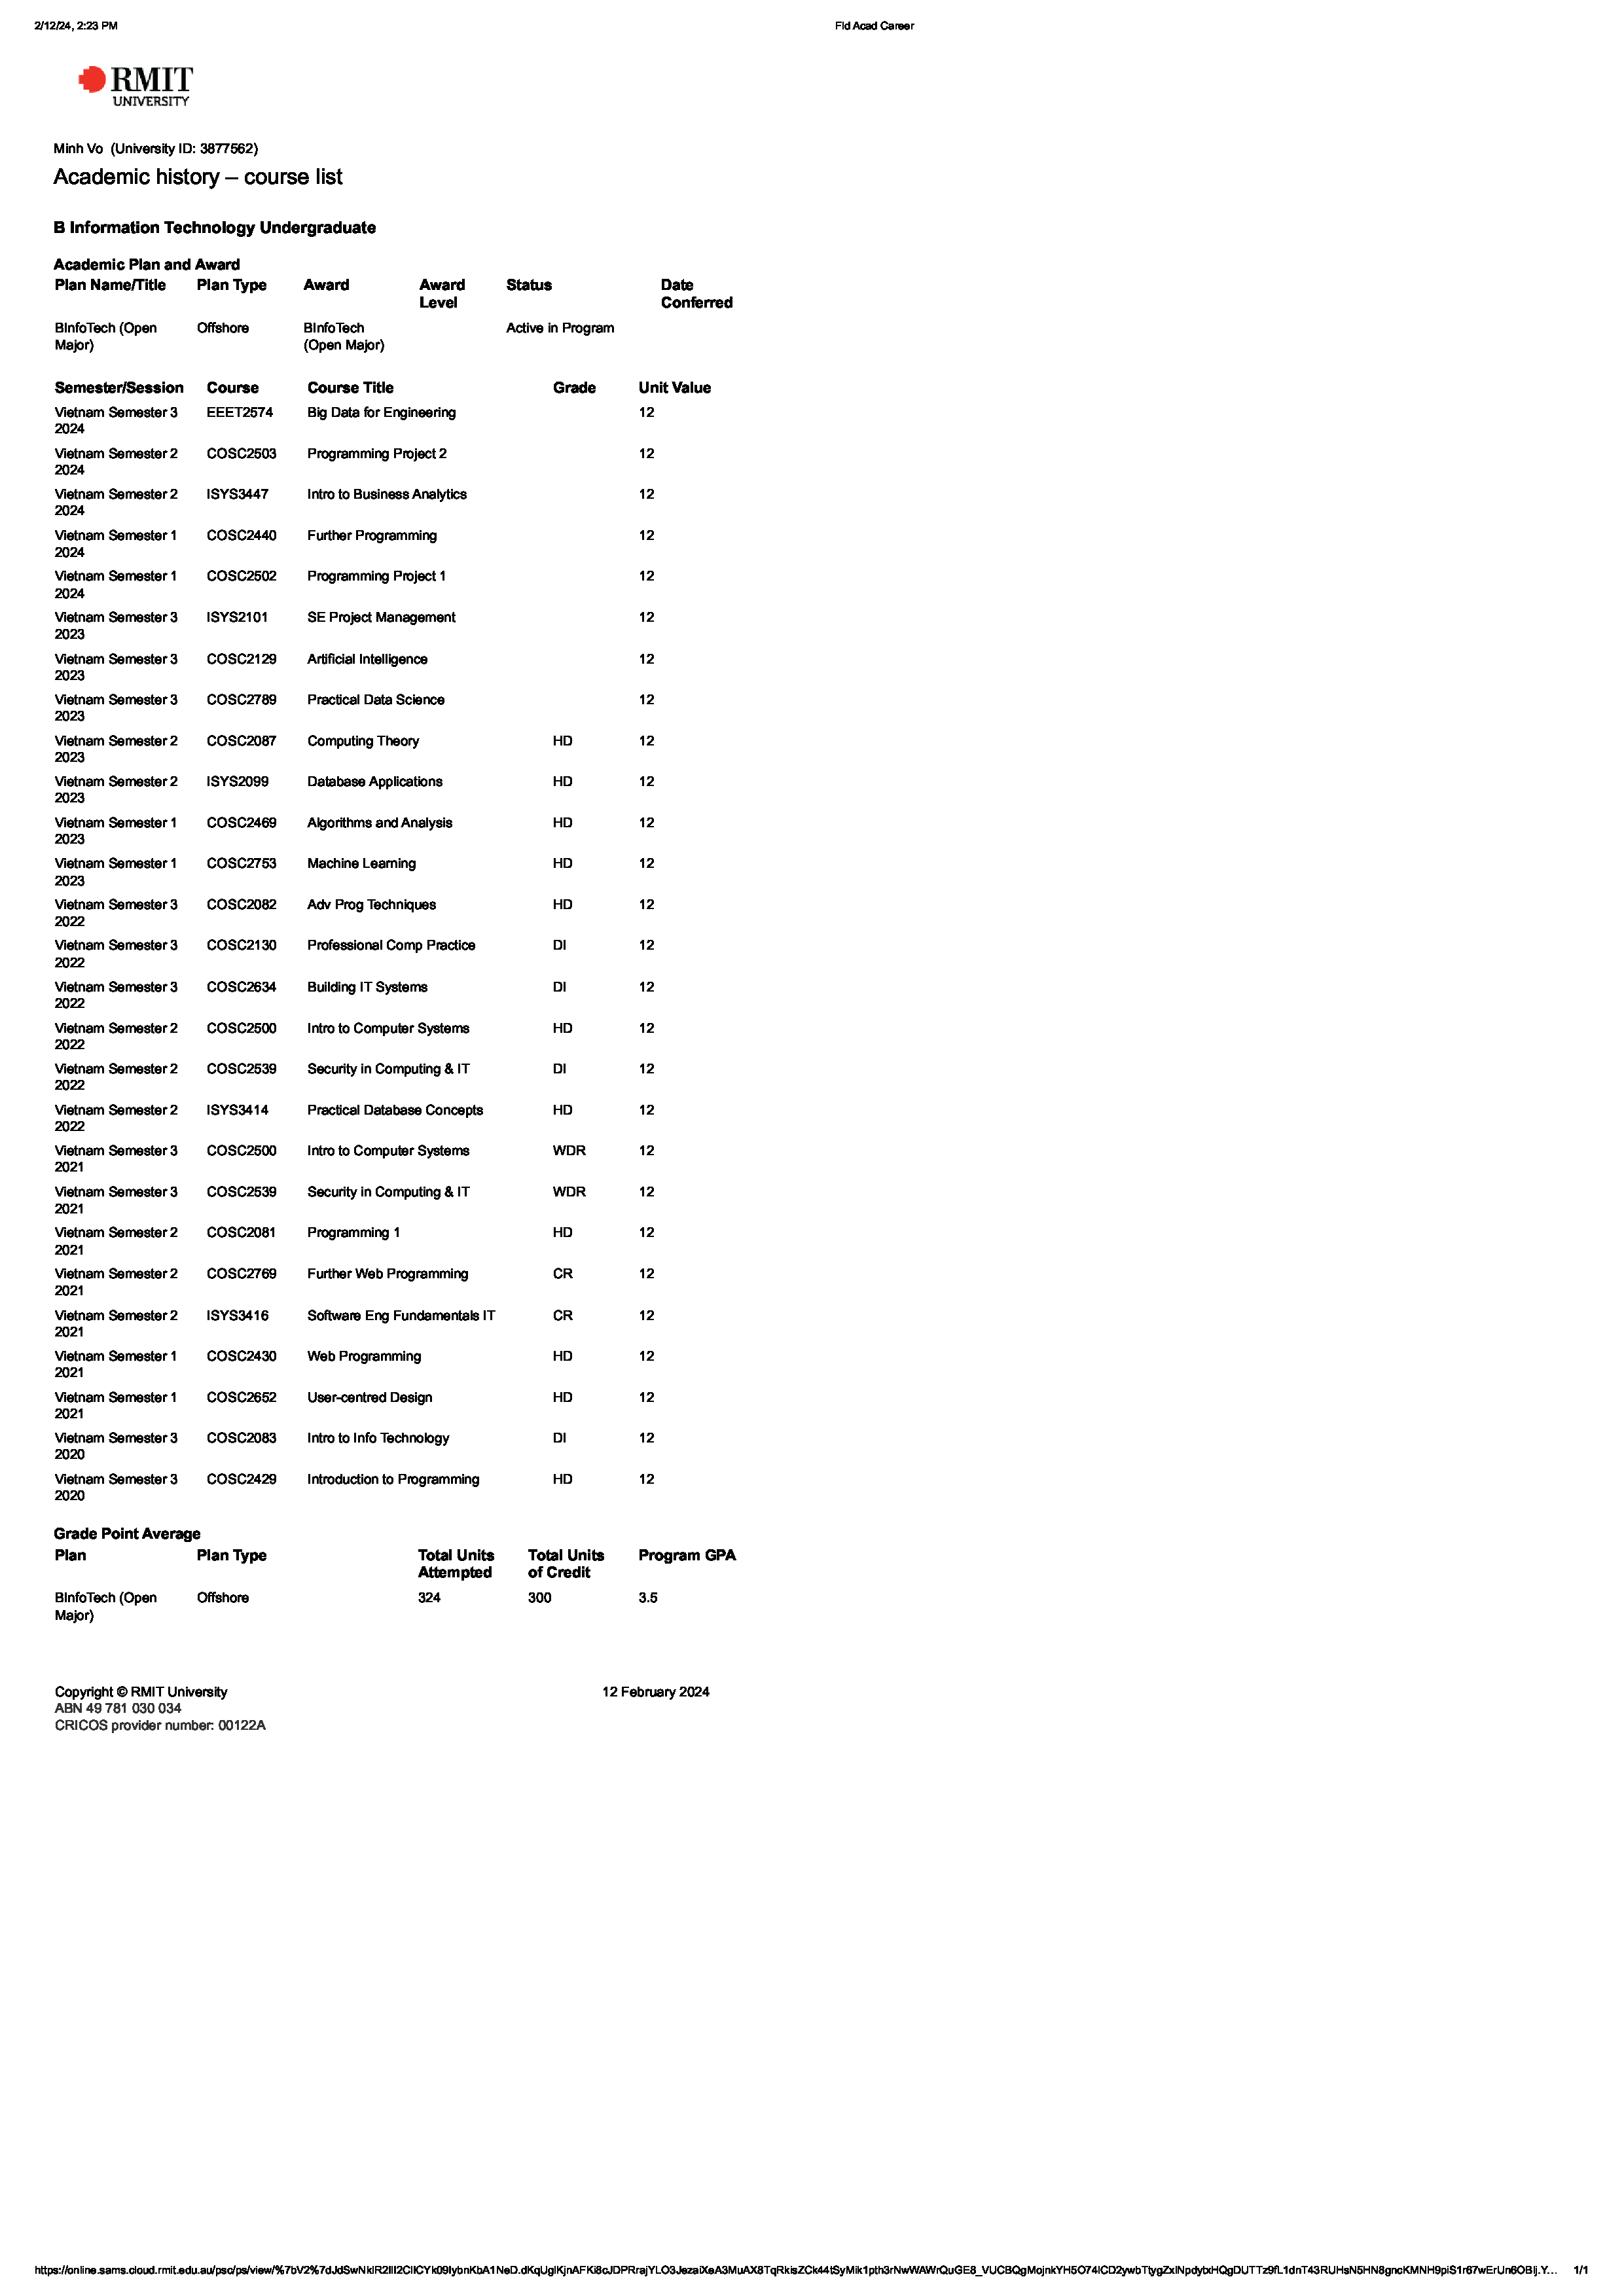
\includepdf[pages=-]{transcript.pdf}
%

% ----- COVER LETTER -----
\coverLetterHeader

\p{\today}

\p{Kính gửi Bộ phận Tuyển dụng,}

\p{Tôi viết thư này muốn bày tỏ sự quan tâm ứng tuyển vị trí Thực tập sinh Kiểm thử Phần mềm E-commerce tại W2Solution Việt Nam. Hiện tại tôi đang theo học chương trình Cử nhân Công nghệ Thông tin chuyên ngành Trí tuệ nhân tạo và Phân tích Dữ liệu tại Đại học RMIT Việt Nam, dự kiến tốt nghiệp đầu năm 2025. Tôi rất phấn khởi với cơ hội được đóng góp kỹ năng và nhiệt huyết của mình cho đội ngũ của công ty.}

\p{Trong quá trình học tập, tôi đã có được nền tảng vững chắc về Phát triển Web, Kiểm thử, Học máy, và Cấu trúc Dữ liệu và Giải thuật. Qua quá trình học tập, tôi hiểu rõ về quy trình phát triển phần mềm, kiểm thử, và tầm quan trọng của documentation. Hơn nữa, tôi luôn tìm cách cải thiện bản thân bằng cách học công nghệ mới và theo kịp xu hướng mới nhất trong ngành.}

\p{Là một người ham học hỏi và có tinh thần đồng đội, tôi đã hoàn thành thành công nhiều dự án khác nhau, từ e-commerce website, web game, đến phần mềm mã nguồn mở. Một trong những nổi bật là đóng góp của tôi trong việc phát triển hai bàn phím ảo Tiếng Việt Mở cho bộ gõ Keyman. Hợp tác với các developer, admin, và cộng đồng người dùng Keyman qua GitHub, tôi đã phát triển, kiểm thử, triển khai và duy trì hai bàn phím Tiếng Việt Telex và VNI. Tính đến 2024, cả hai phiên bản này tổng cộng đã đạt được sự quan tâm đáng kể với hơn 35,000 lượt tải xuống trên trang web của Keyman. Nhờ đó, tôi đã nâng cao kỹ năng làm việc trong môi trường quốc tế với trú trọng ở khả giao tiếp với stakeholder, tư duy phân tích, khả năng ứng nghi và giải quyết vấn đề độc lập.}

\p{Cảm ơn công ty đã dành thời gian xem xét đơn ứng tuyển của tôi. Tôi mong sẽ có cơ hội được đóng góp và học hỏi tại W2Solution Việt Nam.}

\p{Trân trọng,\\
Tường-Minh (Mike) Võ}
%

\end{document}
% ============================================== %
